\documentclass[11pt]{beamer}
\usetheme{Dresden}
\usecolortheme{dolphin}
\graphicspath{{./images/}}
\usepackage[utf8]{inputenc}
\usepackage{pifont}
\usepackage{amsmath}
\usepackage{amsfonts}
\usepackage{amssymb}
\author{Xiaoyu Yin}
\title{Translating Natural Language to SPARQL}
\setbeamercovered{transparent} 
%\setbeamertemplate{footline}[frame number]
%\setbeamertemplate{navigation symbols}{} 
\setbeamertemplate{bibliography entry title}{}
\setbeamertemplate{bibliography entry location}{}
\setbeamertemplate{bibliography entry note}{}
%\logo{} 
\institute[International Center for Computational Logic]
{
International Center for Computational Logic\\
Technische Universität Dresden
} 
\date{8th January 2019} 
%\subject{Master Thesis} 
\begin{document}

\AtBeginSection[]
{
    \begin{frame}
    \frametitle{Outline}
    \tableofcontents[currentsection]
    \end{frame}
}

\begin{frame}
    \titlepage
\end{frame}

\begin{frame}
    \frametitle{Outline}
    \tableofcontents[hideallsubsections]
\end{frame}

\section{Introduction}

\subsection{Motivation}

\begin{frame}{Transformation of the Web}{Motivation}

    \begin{columns}

    \column{0.5\textwidth}
        \begin{block}{Web}
        \begin{itemize}
        \item Linked web pages
        \item Made for human to browse
        \end{itemize}
        \end{block}
    \pause
    \column{0.5\textwidth}
        \begin{block}{Semantic Web}
        \begin{itemize}
        \item Built on the existing Web
        \item Linked knowledge graphs and data
        \item For human and machines to lookup
        \end{itemize}
        \end{block}

    \end{columns}

\end{frame}

\subsection{Background}

\begin{frame}{Semantic Web Technologies}
    \begin{figure}[h]
    \includegraphics[width=0.6\textwidth]{Semantic-web-stack}
    \centering
    \caption{Semantic Web technology stack}
    \label{figure:semantic web stack}
    \end{figure}
\end{frame}

\begin{frame}{Linked Data}
    \begin{itemize}
        \item a notion in Semantic Web
        \item based on RDF 
        \item currently only in commercial applications but has great potentials
    \end{itemize}

    \begin{example}
        \textit{Google Knowledge Graph}
        \textit{DBpedia}
        \begin{itemize}
            \item knowledge from the Wikipedia articles in RDF files so that machines can process easily, open to everyone
        \end{itemize}
    \end{example}
\end{frame}

\begin{frame}{SPARQL}

    \begin{itemize}
        \item like SQL but for the Semantic Web and Linked Data
        \item structured query language
        \item the meaning of a SPARQL query can be usually expressed in Natural Language
        \item Why not Natural Language to SPARQL?
    \end{itemize}

    \begin{block}{Application}
        \begin{itemize}
            \item Broaden the accessibility of the Semantic Web resources
            \item Chatbots, service agents
        \end{itemize}
    \end{block}

\end{frame}

\begin{frame}{Natural Language to SPARQL}
    \begin{itemize}
        \item proved possible by Neural SPARQL Machine (NSpM) \cite{Soru2018a}
        \item no large number of tests have been done before
    \end{itemize}

    \begin{block}{Our goal}
        Conduct a large number of tests on the possibility of translating human language to SPARQL (machine language)
    \end{block}
\end{frame}

\begin{frame}{Machine Translation}{Background}

    \begin{itemize}
        \item Rule-based Machine Translation
        \item Statistical Machine Translation
        \item Example-based Machine Translation
        \item \textbf{Neural Machine Translation}
        \item Hybrid Machine Translation
    \end{itemize}

    \begin{block}{Neural Machine Translation}
        Given large number of training samples, use deep neural networks to perform end-to-end translation between source and target languages.
    \end{block}
\end{frame}

\begin{frame}{Neural Machine Translation}{Background}
    
    \begin{block}{Why NMT?}
        \begin{itemize}
            \item So far \alert{the best performing} methods in translating between natural languages (e.g. English to German)
            \item Abundant choices of neural networks
            \item Off-the-shelf frameworks to use
        \end{itemize}
    \end{block}
    
    \begin{block}{Challenges}
        \begin{itemize}
            \item SPARQL is not like any Natural Language
        \end{itemize}
    \end{block}

\end{frame}

\begin{frame}{Idea}
    \begin{figure}
        \includegraphics[width=\textwidth]{motivation-overview}
    \end{figure}
\end{frame}

\begin{frame}{Idea}
    \begin{figure}
        \includegraphics[width=0.8\textwidth]{datasets-models}
    \end{figure}
    \begin{figure}
        \includegraphics[width=0.4\textwidth]{motivation-overview}
    \end{figure}
\end{frame}

\section{Methodology}

\subsection{Models}

\begin{frame}{Neural Machine Translation}
    \begin{description}
        \item[2013]<1-> Recurrent Neural Networks (RNN) started
        \item[2014-15]<2-> Attention mechanisms
        \begin{itemize}
            \item great enhancements to RNN 
        \end{itemize} 
        \item[2016]<3-> Google Translate System (GNMT)
        \begin{itemize}
            \item bi-directional RNN, residual connection, etc.
        \end{itemize} 
        \item[2017-now]<4-> Convolutional Neural Networks (CNN), Self-attention models joined
        \begin{itemize}
            \item right now state-of-the-art
        \end{itemize} 
    \end{description}
\end{frame}

\begin{frame}{Neural Machine Translation Models}
    \begin{itemize}
        \item Three categories
    \end{itemize}
    \begin{table}
        \begin{tabular}{p{3cm}|p{3cm}|p{3cm}}
            Recurrent Neural Network (RNN) models &  Convolutional Neural Network (CNN) models & Self-Attention models \\
            \hline
            \includegraphics[width=3cm]{rnn-encoder-decoder} & \includegraphics[width=3cm]{convolutions} & \includegraphics[width=3cm]{multi-attention}\\
            \hline
            GNMT & ConvS2S & Transformer
        \end{tabular}
    \end{table}
\end{frame}

\begin{frame}{Google's Neural Machine Translation System (GNMT)}{RNN-based}
    \begin{figure}[h]
        \includegraphics[width=0.9\textwidth]{gnmt-architecture}
        \centering
        \caption{The model architecture of GNMT \cite{Wu2016}.}
        \label{figure:gnmt architecture}
    \end{figure}
\end{frame}

\begin{frame}{Convolutional Sequence-to-Sequence (ConvS2S)}{CNN-based}
    \begin{figure}[h]
        \includegraphics[width=0.3\textwidth]{convs2s-architecture}
        \centering
        \caption{The demonstration of training the Convolutional Sequence-to-Sequence model \cite{gehring2017convs2s}}
        \label{figure:convs2s model}
    \end{figure}
\end{frame}

\begin{frame}{The Transformer}{Self-attention Models}
    \begin{figure}[h]
        \includegraphics[width=0.3\textwidth]{transformer-architecture}
        \centering
        \caption{The architecture of the Transformer model \cite{Vaswani2017}}
        \label{figure:transformer model}
    \end{figure}
\end{frame}

\begin{frame}{Models Summary}
    Out of these three categories, we constructed 8 models...
    \begin{itemize}
        \item RNN-based models: \textbf{NSpM, NSpM+Att1, NSpM+Att2, LSTM\_Luong, GNMT-4, GNMT-8}
        \item CNN-based model: \textbf{ConvS2S}
        \item Self-attention model: \textbf{Transformer}
    \end{itemize}
    \medskip

    \begin{itemize}
        \item NSpM: Basic 2-layer RNN
        \item NSpM+Att: NSpM with attention module
        \item LSTM\_Luong: a deep 4-layer RNN
    \end{itemize}
    
\end{frame}

\subsection{Datasets}

\begin{frame}{Datasets}
    \begin{itemize}
        \item The \textbf{Monument} dataset 
        \item Largescale Complex Question Answering Dataset (\textbf{LC-QUAD})
        \item DBpedia Neural Question Answering (\textbf{DBNQA})
    \end{itemize}
    \pause
    \begin{table}
        \begin{tabular}{|c|c|c|c|}
            \hline
            & Monument & LC-QUAD & DBNQA \\
            \hline
            Instance & 14,788 & 5,000 & 894,499 \\
            \hline
            English vocab & 2,500 & 7,000 & 131,000 \\
            \hline
            SPARQL vocab & 2,200 & 5,000 & 244,900 \\
            \hline
        \end{tabular}
        \caption{Sizes of three used English-SPARQL datasets}
    \end{table}
\end{frame}


\subsection{Metrics}

\begin{frame}{Evaluation Metrics}
    \begin{itemize}
        \item \textbf{Perplexity} for training phase
        \item \textbf{BLEU} for testing phase
    \end{itemize}
    \only<1>{
        \begin{block}{Perplexity}
            \begin{itemize}
                \item 1 $ \rightsquigarrow $ +$\infty $
                \item reflects how well the model is trained (1 is best)
            \end{itemize}
        \end{block}
    }
    \only<2>{
        \begin{block}{BLEU}
            \begin{itemize}
                \item 0 $ \rightsquigarrow $ 100
                \item reflects the quality of the generated translations compared to the reference (100 is best)
                \item widely used in Machine Translation tasks
            \end{itemize}
        \end{block}
    }
    \only<3->{
        \begin{example}[BLEU]
            \begin{description}
                \item[Translation] the cat sat on the mat
                \item[Reference 1] there is a cat on the mat
                \item[Reference 2] the cat is on the mat
            \end{description}
            BLEU Score: \alert{42}
        \end{example}
    }
    
\end{frame}

\section{Experiments}

\begin{frame}{Experiment Overview}

    \begin{figure}
        \includegraphics[width=0.9\textwidth]{experiment_overview}
    \end{figure}

\end{frame}

\begin{frame}{Dataset Preprocessing}
    
    \only<1>{
        \begin{block}{Dataset Splitting}
            \begin{itemize}
                \item Split the Monument, LC-QUAD, and DBNQA into 80\%/10\%/10\% training/validation/testing set
                \item Split the Monument dataset further into 50\%/10\%/40\% and 14588/100/100 (in NSpM paper)
                \item Leads to 5 different splits: \textbf{MonumentNSpM, Monument50, Monument80, LC-QUAD, DBNQA}
            \end{itemize}
        \end{block}
    }

    \only<2>{
        \begin{block}{SPARQL Encoding}
            \includegraphics[width=\textwidth]{sparql-encoding}
        \end{block}
    }

\end{frame}

\begin{frame}{Hardware}

    \begin{table}[h]
        \small
        \centering
        \begin{tabular}{|c|p{2cm}|p{3cm}|p{2cm}|}
            \hline
            & GPU \textbf{Small} & GPU \textbf{Medium} & GPU \textbf{Large} \\
            \hline
            CPU & Intel\textsuperscript{\textregistered} Xeon\textsuperscript{\textregistered} CPU E5-2450 @ 2.10GHz & Intel\textsuperscript{\textregistered} Xeon\textsuperscript{\textregistered} CPU E5-2680 @ 2.50GHz & POWER9  \\
            \hline
            RAM & 24 GB & 16 GB & 192 GB \\
            \hline
            Cores & 8 & 6 & 32 \\
            \hline
            \alert{GPU} & NVIDIA\textsuperscript{\textregistered} Tesla\textsuperscript{\textregistered} K20Xm & NVIDIA\textsuperscript{\textregistered} Tesla\textsuperscript{\textregistered} K80 & NVIDIA\textsuperscript{\textregistered} Tesla\textsuperscript{\textregistered} V100-SXM2 \\
            \hline
            \alert{GPU RAM} & 6 GB & 12 GB & 32 GB \\
            \hline
        \end{tabular}
        \caption{Three hardware configurations on High Performance Computing (HPC) server used in this thesis}
        \label{table:hpc gpus}
    \end{table}

\end{frame}

\begin{frame}{Software (1/2)}
    \begin{block}{Python Frameworks}
    \begin{itemize}
        \item \textit{nmt}\footnote{\url{https://github.com/tensorflow/nmt}} based on TensorFlow
        \begin{itemize}
            \item Implements: \textbf{NSpM, NSpM+Att1, NSpM+Att2, GNMT-4, GNMT-8}
        \end{itemize}
        \item \textit{fairseq}\footnote{\url{https://github.com/pytorch/fairseq}} based on PyTorch
        \begin{itemize}
            \item Implements: \textbf{LSTM\_Luong, ConvS2S, Transformer}
        \end{itemize}
    \end{itemize}
    \end{block}
    Takes care of training, validation, and testing the models on given dataset and outputs the results and statistics
\end{frame}

\begin{frame}{Software (2/2)}
    \begin{block}{Operating Systems}
        \begin{itemize}
            \item \includegraphics[height=12pt]{linux} Linux from HPC with Python 3.6.4, TensorFlow 1.8.0, and PyTorch 0.4.1
            \begin{itemize}
                \item Ran the training and testing jobs and saved the results
            \end{itemize}
            \item \includegraphics[height=12pt]{apple} macOS High Sierra 10.13.6 from my computer with Python 3.6.5, TensorFlow 1.8.0, PyTorch 0.4.1, and matplotlib 3.0.2
            \begin{itemize}
                \item Preprocessed the datasets
                \item Uploaded and downloaded jobs between HPC
                \item Analyzed the outputs
            \end{itemize}
        \end{itemize}
    \end{block}
    Source code is all available on GitHub\footnote{\url{https://github.com/xiaoyuin/tntspa}}.
\end{frame}

\subsection{Experimental Setups}

\begin{frame}{Hyperparameters}
    Tricky part of neural network training
    \medskip
    \begin{enumerate}
        \item Adopted recommended hyperparameters from each framework
        \item Adjusted for the \textbf{MonumentNSpM} dataset split
        \item Applied on the other splits
    \end{enumerate}
\end{frame}

\section{Results \& Discussion}

\begin{frame}{Results}
    For each dataset split and model, we report...
    \begin{itemize}
        \item \textbf{Perplexity graphs} on the training and validation set
        \item \textbf{BEST BLEU} on the test set
    \end{itemize}
    \medskip\medskip
    In total, 5 (dataset splits) * 8 (models) = 40 perplexity graphs and 40 BLEU scores
\end{frame}

\begin{frame}{Results}
    \begin{example}
        \begin{columns}

            \column{0.5\textwidth}
            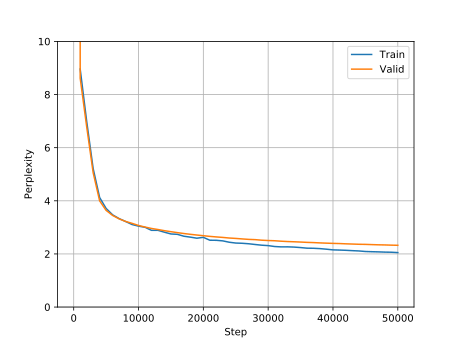
\includegraphics[width=\textwidth]{../results/dbnqa1/run1/neural_sparql_machine/ppls.png}
            \column{0.5\textwidth}
            \begin{table}
                \tiny
                \begin{tabular}{c|c|c}
                    Models & \textbf{Test BLEU} & Step / Epoch \\
                    \hline
                    NSpM & 65.92 & Step 50k \\
                    NSpM+Att1 & 89.87 & Step 50k \\
                    NSpM+Att2 & 91.50 & Step 50k \\
                    GNMT-4 & 69.61 & Step 30k \\
                    GNMT-8 & 68.41 & Step 30k \\
                    LSTM\_Luong & 77.67 & Epoch 55 \\
                    ConvS2S & \textbf{96.07} & Epoch 54 \\
                    Transformer & 68.82 & Epoch 53 \\
                \end{tabular}
            \end{table}
            \end{columns}
    \end{example}
\end{frame}

\begin{frame}{Dataset Comparison}

    \pause
    Three different splits of the monument dataset did not show very big differences in results
    \begin{itemize}
        \item The \textbf{Monument} dataset is relatively simple
    \end{itemize}

    \pause
    Serious overfit in LC-QUAD dataset experiments
    \begin{itemize}
        \item The \textbf{LC-QUAD} dataset is too small in size
    \end{itemize}

    \pause
    \begin{itemize}
        \item The \textbf{DBNQA} is so far the most suitable for this task
    \end{itemize}
    \medskip
    \pause
    But they are all relatively simpler compared to Natural Language datasets
    \begin{itemize}
        \item \alert{25-30 BLEU} for Natural Language task, \alert{60-100 BLEU} for our task
    \end{itemize}
\end{frame}

\begin{frame}{Model Comparison}

    \begin{itemize}
        \item<1> \textbf{ConvS2S} model outperformed other models in converging speed (Perplexity curves) and translation quality (BLEU scores)
        \item<2> Attention mechanisms contributed to the translation quality
        \item<3> GNMT (deeper-layer model) performs relatively worse than shallower-layer models
        \item<4> The Transformer model is relatively harder to train
    \end{itemize}

\end{frame}

\begin{frame}{Perplexity vs. BLEU}
    \begin{figure}
        \includegraphics[width=0.7\textwidth]{perplexity-bleu}
        \centering
        \caption{The perplexity-BLEU graph on the validation set in the DBNQA experiments}
    \end{figure}
\end{frame}

\begin{frame}{Limitations}

    \begin{block}{Training}
        \begin{itemize}
            \item Training hyperparameters are not tuned specifically for each model and each dataset.
            \item Framework differences
        \end{itemize}
    \end{block}

    \begin{block}{Testing}
        \begin{itemize}
            \item BLEU is not a perfect metric for SPARQL
        \end{itemize}
    \end{block}

\end{frame}

\section{Summary \& Outlook}

\begin{frame}{Summary \& Outlook}
    \begin{itemize}
        \item Semantic Web and SPARQL
        \item Neural Machine Translation Models
        \item Experiments
        \item Results and Discussion
        \pause
    \end{itemize}
    \begin{block}{Future Work}
        \begin{itemize}
            \item a better NL-SPARQL dataset
            \item better metric instead of BLEU
            \item more hyperparameter tuning
        \end{itemize}
    \end{block}
\end{frame}

\begin{frame}
\begin{center}
    \begin{LARGE}
        Thank you !
    \end{LARGE}
\end{center}
\end{frame}

\begin{frame}{Reference}
\bibliographystyle{amsalpha}
\bibliography{literature}
\end{frame}

\end{document}
    
